\chapter{Exercises}
The exercises included in this chapter span over multiple chapters or are no longer required by the syllabus.
\begin{enumerate}
\item{[SC 2002/11 SG] Which one of the following combinations contains one SCALAR and one VECTOR quantity?
\begin{enumerate}
\item momentum and force
\item displacement and acceleration
\item potential difference and electric field strength
\item resistance and electric current
\end{enumerate}}

\item{[DOE 2005/11 SG1] Which one of the following pairs consists of two vector quantities?
\begin{enumerate}
\item time, acceleration
\item velocity, displacement
\item electric field strength, charge
\item momentum, kinetic energy.
\end{enumerate}}

\item{[IEB 2004/11 HG1] Which one of the following is not equivalent to the SI unit of energy?
\begin{enumerate}
\item{N.s}
\item{N.m}
\item{V.C}
\item{W.s}
\end{enumerate}
}

\item{[IEB 2002/11 HG1 - Electrostatics] \textbf{Millikan's Oil Drop Experiment}\\
The diagram below represents the apparatus used to measure the charge carried by oil droplets. The droplets are sprayed above the top plate and eventually a single droplet finds its way through a small hole into the space between the plates.

\begin{center}
\begin{pspicture}(0,0)(5,5)
\psgrid[gridcolor=lightgray]
\end{pspicture}
\end{center}

The mass of the droplet is m and it carries a negative charge of magnitude q. The distance between the plates is d. The oil droplet between the two plates is stationary.

\begin{enumerate}
\item{Use expressions for the electric field intensity and weight to derive a formula for the charge carried by the oil droplet.}
\item{In one particular experiment, a student reported that, while using a voltage of 400 V between the plates, she had obtained a value of 4,8 $\times$ 10$^{-19}$ C for the charge on the oil droplet. Another student said that he had repeated the same experiment with the same oil droplet but that he had used 800 V to keep the oil droplet stationary. If this were true, what would be the charge on the oil droplet, and why would you doubt what he had reported?}
\end{enumerate}}

\item{[IEB 2004/11 HG1] An electric motor lifts a load of mass m through a vertical height h at a steady speed of v. It is connected to a power supply of potential difference V, and it draws a current I. Assume that 90\% of the energy input is transferred to useful work done, and that the load comes to rest at the top of this height h.


Which expression correctly relates the power input to the power output for this system?

\begin{enumerate}
\item{VI = (0,9)mgh}
\item{VI = (0,9)mgv}
\item{(0,9)VI = mgh}
\item{(0,9)VI = mgv}
\end{enumerate}}
\end{enumerate}

% CHILD SECTION END 



% CHILD SECTION START 

\part{Essays}

% CHILD SECTION START 

\essay[Energy and electricity. Why the fuss?]

\essayauthor[Asogan Moodaly]

\essayauthorblurb[Asogan Moodaly received his Bachelor of Science
degree (with honours) in Mechanical Engineering from the University
of Natal, Durban in South Africa. For his final year design project
he worked on a 3-axis filament winding machine for composite (Glass
re-enforced plastic in this case) piping. He worked in Vereeniging,
Gauteng at Mine Support Products (a subsidiary of Dorbyl Heavy
Engineering) as the design engineer once he graduated. He currently
lives in the Vaal Triangle area and is working for Sasol Technology
Engineering as a mechanical engineer, ensuring the safety and
integrity of equipment installed during projects.]

Disclaimer: The details furnished below are very basic and for
illustration purposes only.

Why do we need energy? Note that I use the word 'energy' and not
'electricity'. On a broad scale it stimulates economic growth, etc,
etc but on a personal level it allows us to lead a comfortable
lifestyle.

e.g. Flick a switch and… 
\begin{itemize}
\item Heat for cooking 
\item Entertainment such as television and radio 
\item Heat for water and interior of house 
\item Ironing
\item Electronic and electrical devices such as alarms, garage doors, etc.
\end{itemize}

In a modern household this energy is provided in the form of electricity which is powered via fossil fuels or nuclear.

How is electricity made? In a nutshell: By moving a magnet through or near a set of conducting coils.

\begin{figure}[H]
\centering
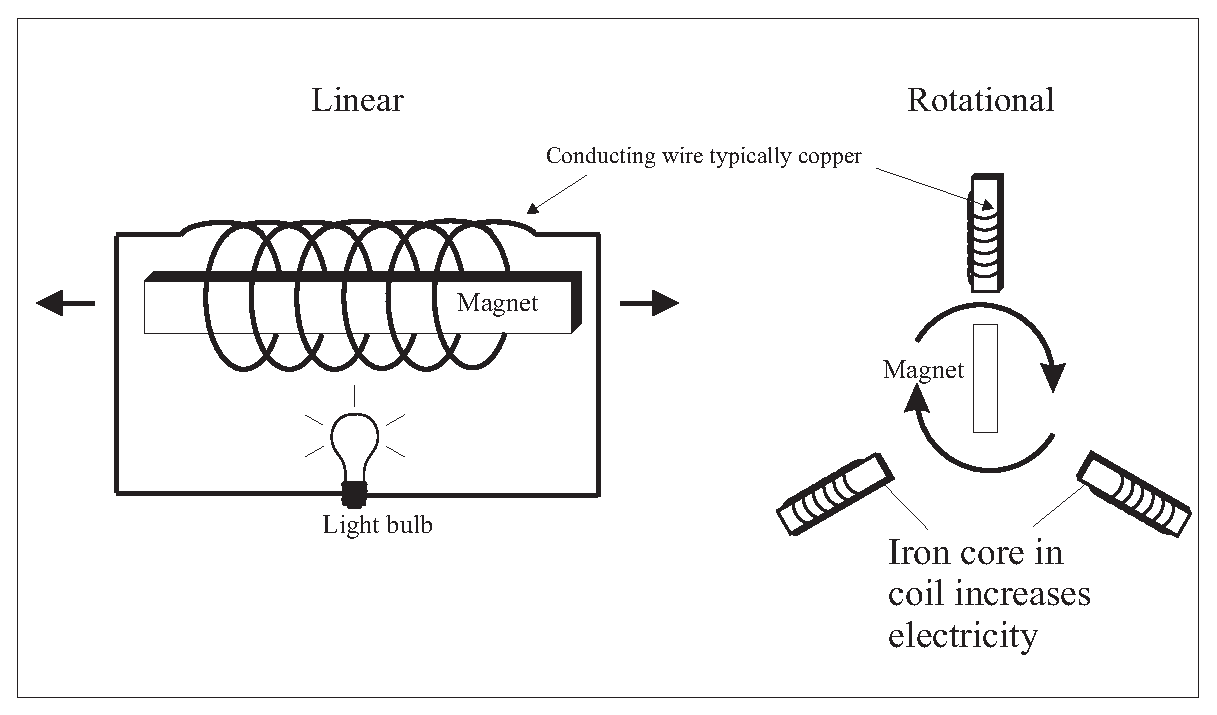
\includegraphics[scale=0.4]{../../epsimages/1ElectricityGeneration.eps}
\end{figure}

Most power stations produce steam through heat (nuclear reaction or burning fossil fuels), the steam drives a turbine which moves a magnet relative to a coil (the generator - like the above but on a much larger scale i.e. bigger magnets, bigger coils, etc), which produces electricity that is transmitted via a power network to our homes. Gas fired plants burn gas directly in a gas turbine to produce the same desired relative motion between permanent magnet and coil.

\begin{figure}[H]
\centering
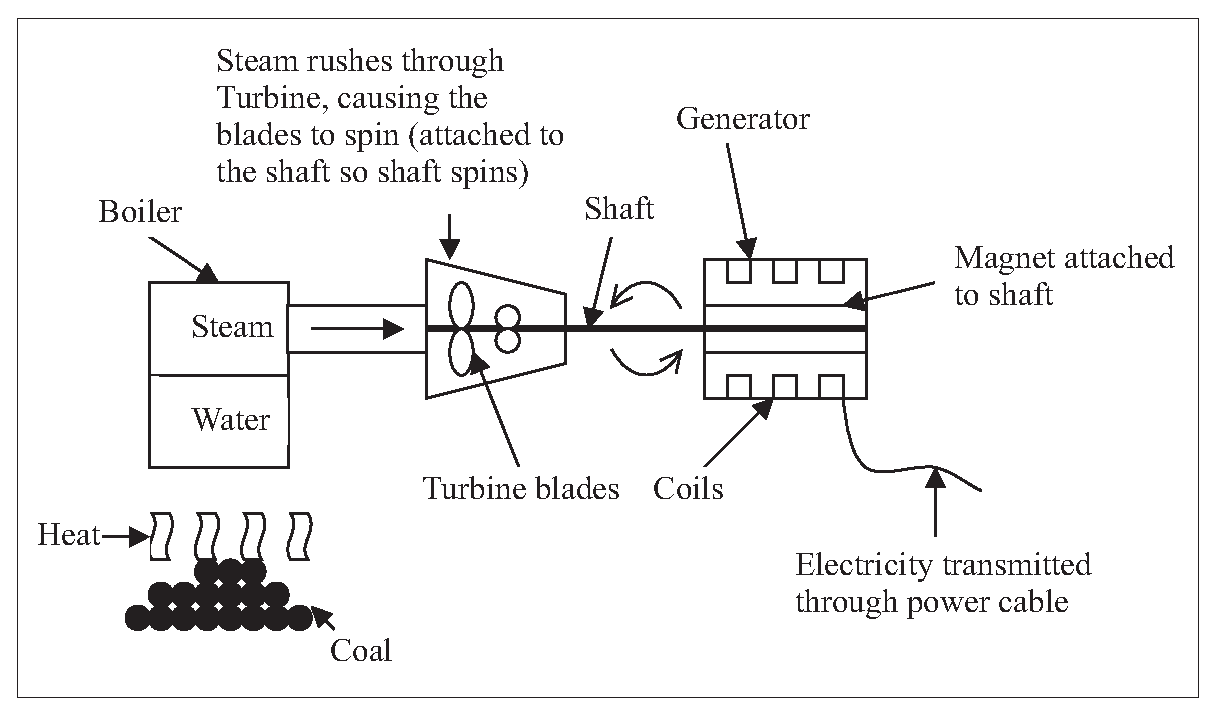
\includegraphics[scale=0.4]{../../epsimages/2SteamPower.eps}
\end{figure}

\begin{figure}[H]
\centering
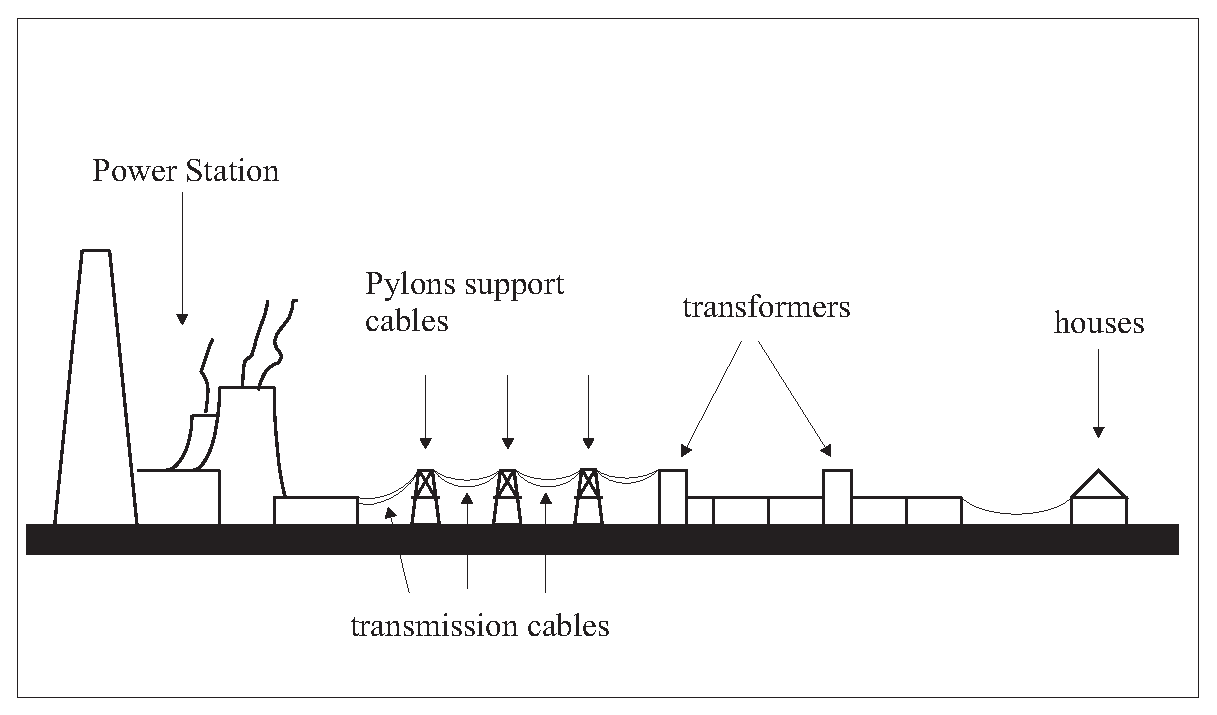
\includegraphics[scale=0.4]{../../epsimages/3PowerStation.eps}
\end{figure}

Coal, oil and gas are fossil fuels. Fossil fuels were created by
decomposing organic (plant and animal) matter a long, long time ago
and are typically found underground. Different temperatures and
pressures resulted in the organic matter transforming into coal, oil
or gas.

Why the fuss about fossil fuels?
\begin{enumerate}
\item Fossil fuel power is bad news in
the long run. It pollutes and contributes to the greenhouse effect
(global warming resulting in melting polar ice caps, floods,
droughts, disease, etc).
\item It's not going to last forever.
\item Nuclear power is 'cleaner' in terms of emissions but there's no proven way
of disposing of the nuclear waste. Oh, and it won't last forever
either!
\end{enumerate}

Renewable Energy As the name suggests renewable energy lasts
'forever'. Solar (sun), wind, geothermal, wave, hydro and biomass
(organic) are all sources of energy that will last until the sun
eventually explodes many millions of years from now. Hopefully the
human race will have moved from the earth by then! Generally the
principal of renewable electricity generation is similar to fossil
fuel electricity generation in that electricity is generated by
moving a magnet relative to a conducting coil. What is different is
the way energy is supplied to cause that motion.

The below are a few different types of available renewable energy
technologies.

\subsection*{Solar}

There are different types of solar electricity technologies, the
main ones being solar thermal and photovoltaic.

\begin{figure}[H]
\centering
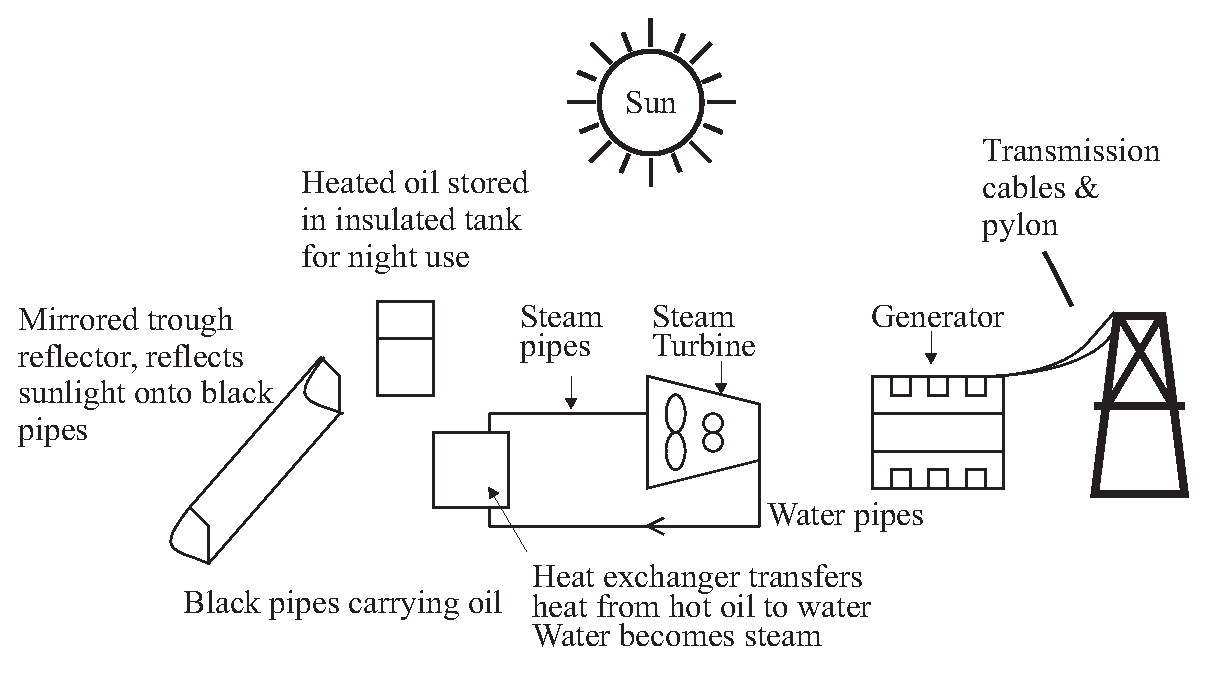
\includegraphics[scale=0.4]{../../epsimages/4solar1.eps}
\end{figure}

Solar thermal uses the heat of the sun to produce electricity. Sun
is concentrated using mirrors. This heat either creates steam which
drives a turbine which in turn drives a generator (as per fossil
fuel generation), or drives an air engine (engine that uses
expanding air to obtain motion) that drives a generator.

Photovoltaic panels convert sunlight directly into electricity. The
benefit of photovoltaic panels is that there are no moving parts,
and is therefore relatively maintenance free. The downside is that
it's very expensive at this stage (17/06/2004).

\begin{figure}[H]
\centering
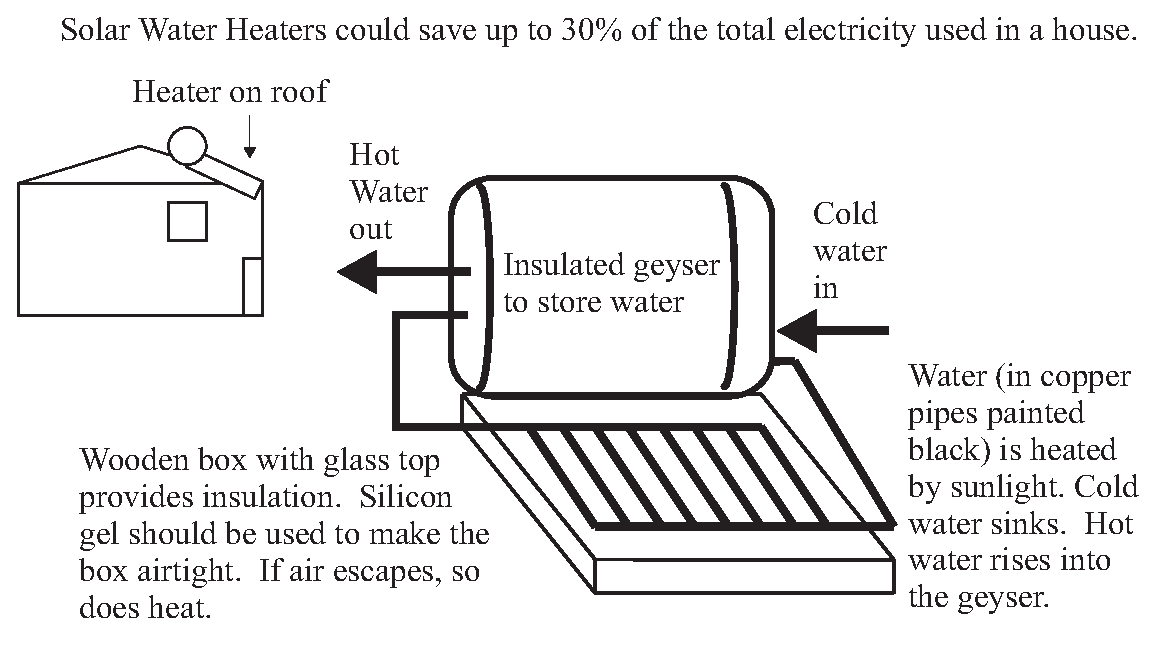
\includegraphics[scale=0.4]{../../epsimages/4solar2.eps}
\end{figure}

\subsection*{Wind}

Wind turbines catch wind that spins the blades. The blades are
connected to a shaft that spins because of the wind. This spinning
shaft spins another shaft that turns a permanent magnet relative to
conducting coils.

Note that 'gears' are used to convert the slow spinning of the 1st
shaft to a faster spin on the 2nd shaft. The generator shaft needs
to spin at the correct speed to produce the right amount and quality
of electricity. Some generators are now being modified to run at
slower speeds. This saves money as gears are not needed.

\begin{figure}[H]
\centering
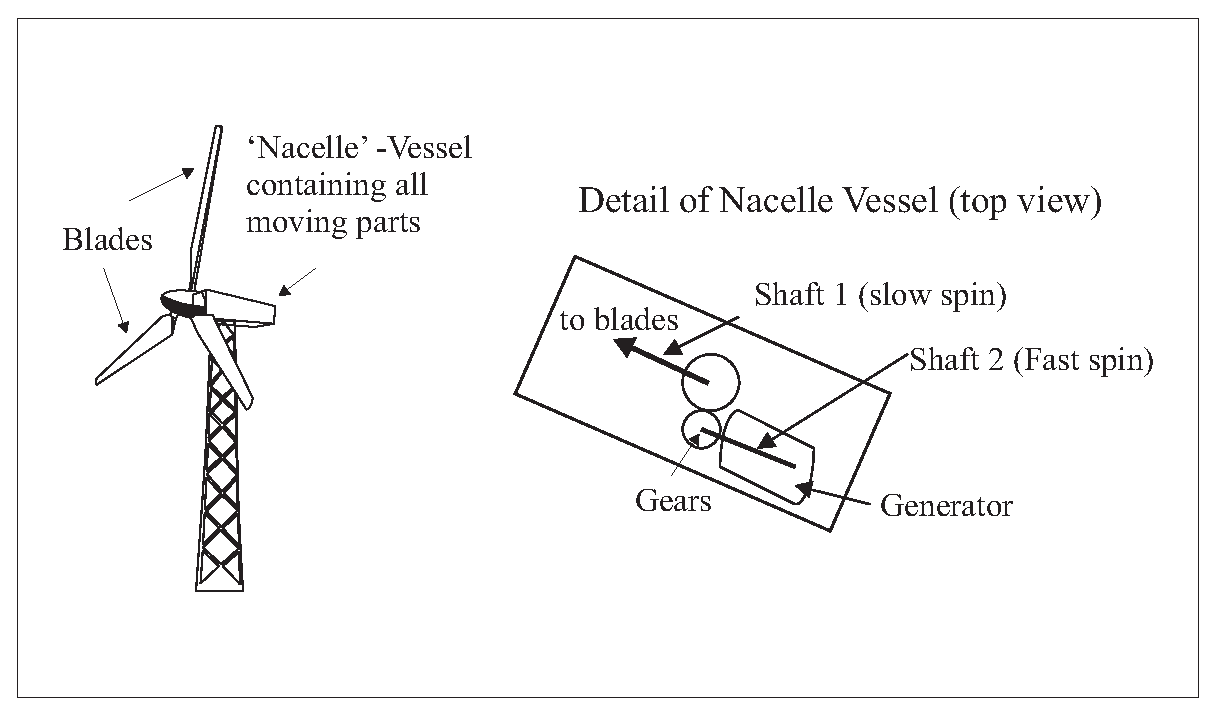
\includegraphics[scale=0.4]{../../epsimages/5Windturbine.eps}
\end{figure}

\subsection*{Biomass}

Biomass is anything organic i.e. plant or animal matter. It can be
used in the place of coal as per a normal coal fired plant and is
renewable as long as the biomass e.g. wood; is handled in a
sustainable manner. By sustainable I mean that suitable farming
practices are used so that the land is not 'over farmed' which will
result in the soil becoming barren and nothing growing there again.

\begin{figure}[H]
\centering
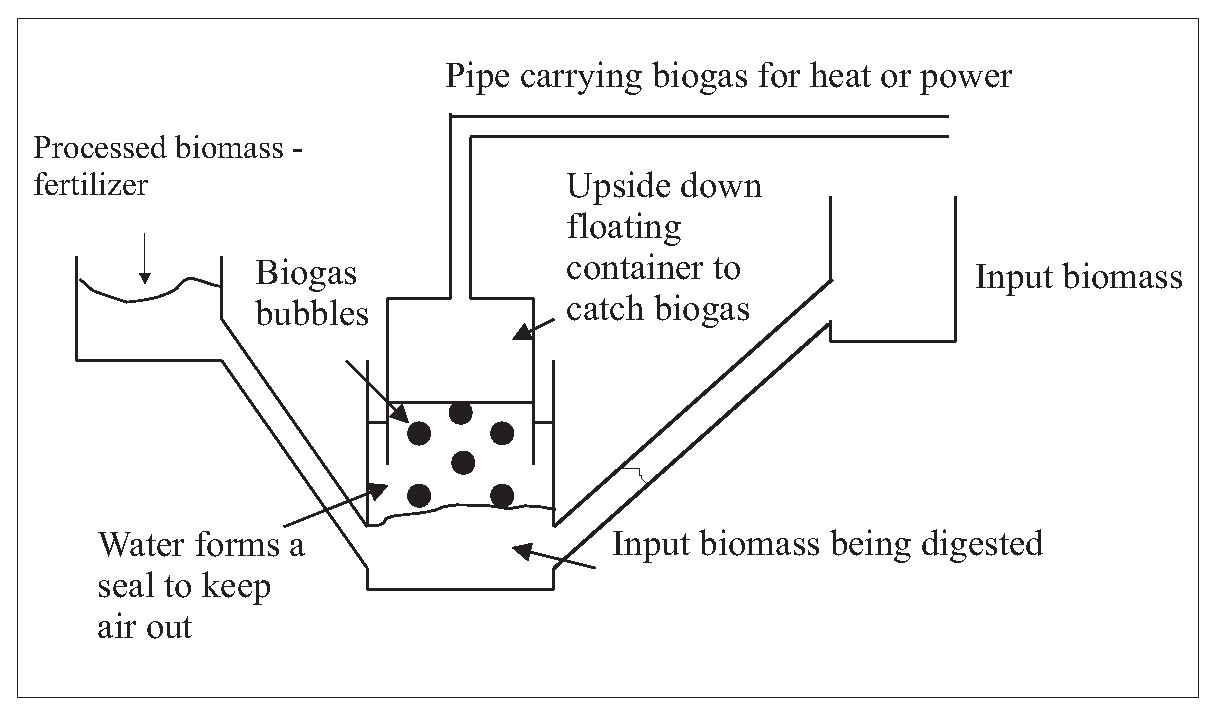
\includegraphics[scale=0.4]{../../epsimages/6biogas.eps}
\end{figure}

Biomass can also be processed using 'anaerobic digestion' to produce a gas that can be burned for heat or electricity. This 'biogas' is made up of a number of other gases that are similar to those found in fossil fuel natural gas - Except the amount of the gases are different. E.g. Natural gas has about 94% methane and biogas has about 60% methane. (Methane is a gas that can be burnt for heat or power)

Anaerobic digestion: 'Anaerobic' means 'No air'. Therefore
'anaerobic digestion' means to digest in the absence of air.
Bacteria that naturally exist in organic matter will convert organic
matter to biogas and fertilizer when all the air is removed.

Thousands of anaerobic digesters have been installed in rural India,
Nepal and China in rural area's where cow dung, human waste and
chicken litter (faeces) are all processed using anaerobic digestion
to produce gas that can be burned in the home for cooking and
heating. The leftover is used as fertilizer.

\subsection*{Geothermal Energy}

In some places on earth, the earth's crust is thinner than others.
As a result the heat from the earth's core escapes. The heat can be
captured by converting water to steam, and using the steam to drive
a steam generator as discussed above.

Hydroelectric power Water from a river is diverted to turn a water
turbine to create electricity similar to the principles of steam
generation. The water is returned to the river after driving the
turbine.

\begin{figure}[H]
\centering
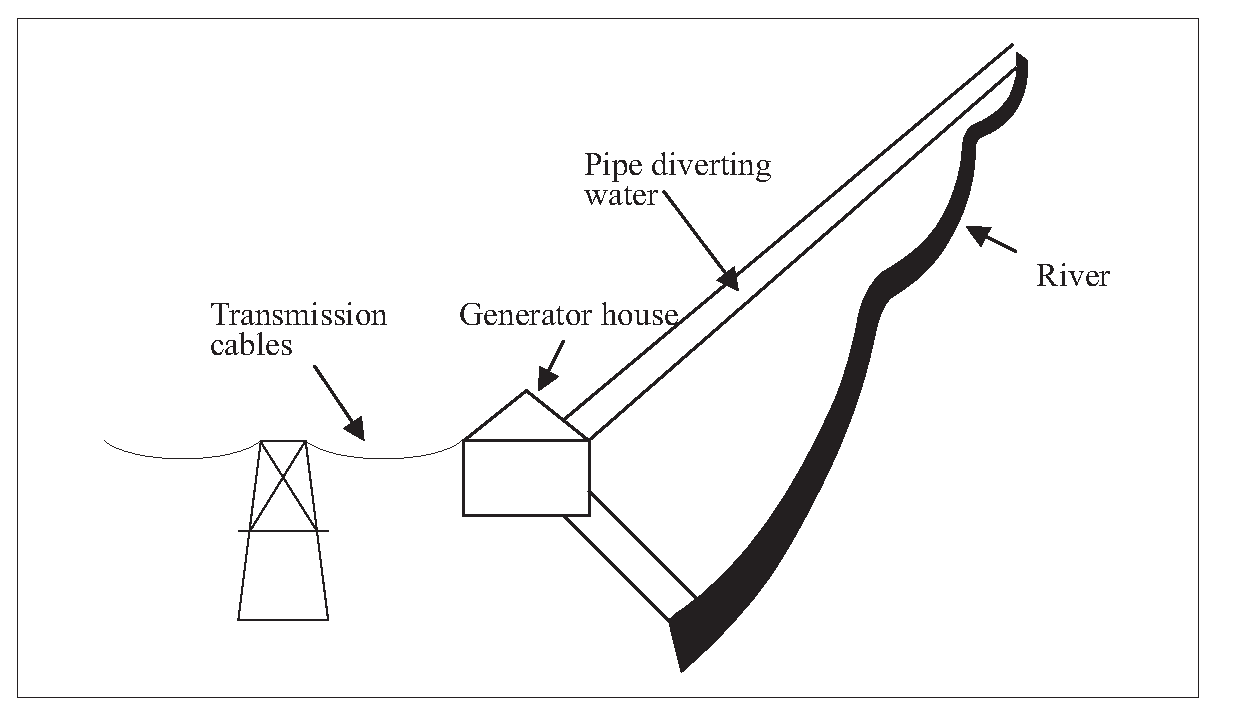
\includegraphics[scale=0.4]{../../epsimages/7hydroelectricriver.eps}
\end{figure}

\subsection*{Wave Energy}

Some wave energy generators work similarly to
wind turbines except that underwater ocean currents turns the blades
instead of wind; and of course most of the structure is under water!
\begin{figure}[H]
\centering
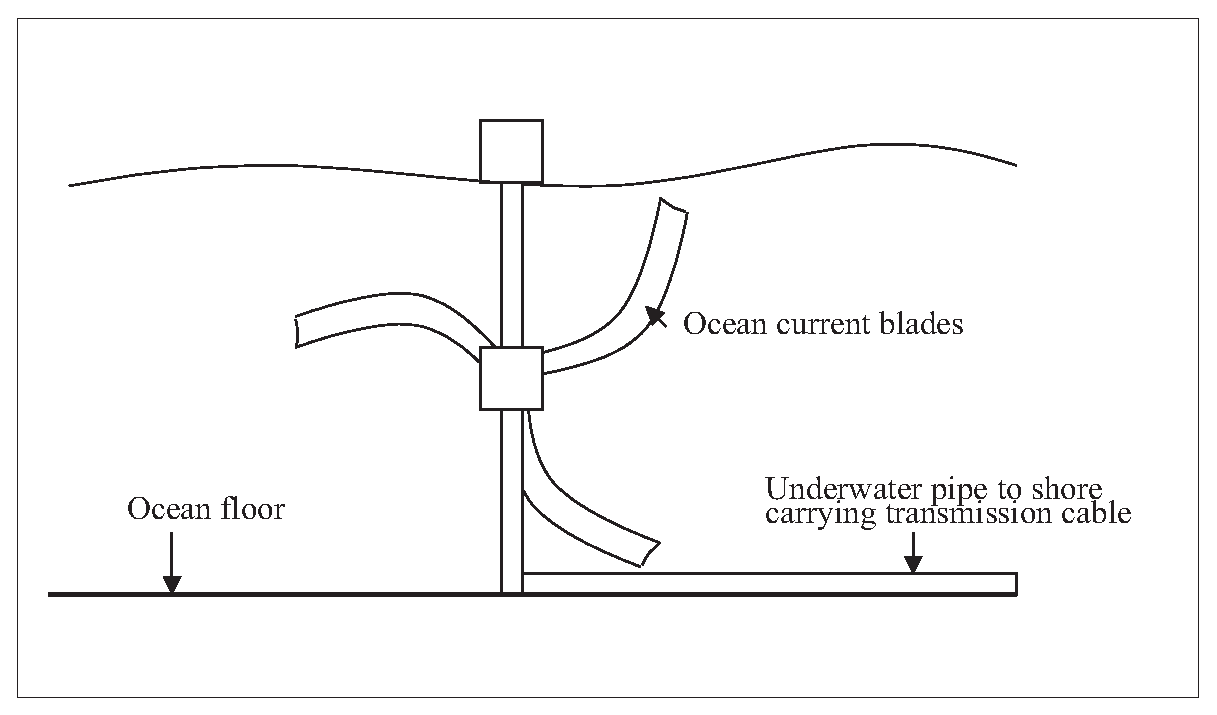
\includegraphics[scale=0.4]{../../epsimages/8hydroelectricocean1.eps}
\end{figure}

Another concept uses the rising and falling of the tides to suck air
in using a 'one way valve'. As a result air becomes compressed in a
chamber and the compressed air is let out to drive a turbine which
in turn drives a generator

\begin{figure}[H]
\centering
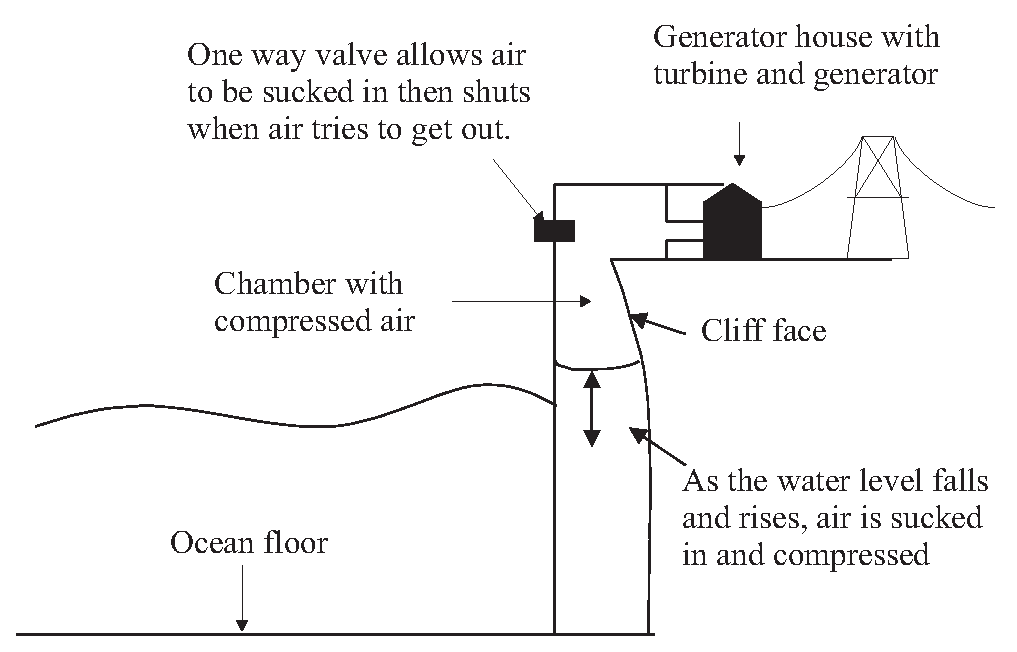
\includegraphics[scale=0.4]{../../epsimages/8hydroelectricocean2.eps}
\end{figure}

These are relatively new technologies.

Liquid Fuels Liquid fuels are used mainly for transportation. Petrol
and diesel are the most common liquid fuels and are obtained from
oil.

Sasol is the only company in the world that makes liquid fuels from
coal; and will be one of the leading companies in the world to make
liquid fuels from natural gas! The Sasol petro-chemical plants are
based in Sasolburg on the border of the Free State and in Secunda in
Mpumalanga.

However, as discussed above coal, gas and oil are fossil fuels and
are not renewable. Petrol and diesel are obtained from fossil fuels
and therefore pollute and contribute to the green house effect
(global warming).

\subsection*{Alternatives}

\subsubsection*{Biodiesel} Oil can be extracted from plants such as the
soya bean, sunflower and rapeseed by pressing it through a filter.
This oil if mixed correctly with either methanol or dry ethanol and
Sodium Hydroxide will separate the plant oil into biodiesel,
glycerol and fertilizer.

The biodiesel can be used as produced in a conventional diesel
engine with little or no modifications required.

The glycerol can be refined a bit further for pharmaceutical
companies to use, or can be used to make soap.

\subsubsection*{Ethanol}

Corn, maize and sugar cane can be used to make ethanol as a fuel
substitute for petrol. It's made by the same fermentation process
used to make alcohol. Enzymes are often used to speed up the
process.

In ethanol from sugar cane production, the leftover 'bagasse' (the
fibre part of the sugar cane) can be burned in a biomass power
station to produce electricity.

\subsubsection*{Hydrogen} Through the process of 'electrolysis'
electricity (hopefully clean, renewable electricity!) can split
water into hydrogen and oxygen. The stored hydrogen can be used in a
'fuel cell' to create electricity in a process that is opposite to
electrolysis; to drive electric motors in a car. The hydrogen can also be burned directly in a modified internal combustion engine. In both cases the 'waste' product is water.



% CHILD SECTION END 



% CHILD SECTION START 

